\subsection{Bloque \textit{Acensor}:}
    
    La interfaz, entradas y salidas, de este bloque se puede ver su representación en la Figura \ref{fig:BloqueIAscensor}:
    
    \begin{figure}[H]
		    \centering
		    \includegraphics[width = 0.8\textwidth ]{BloqueAscensor}
		    \caption{Diagrama Interfaz Bloque PisoActual}
		    \label{fig:BloqueIAscensor}
	\end{figure}
	
	Esta es una entidad de alto nivel que encapsula todo el funcionamiento del ascensor. Se puede ver el diagrama de bloques interno de esta entidad en la siguiente figura: 
	
	\begin{figure}[H]
		    \centering
		    \includegraphics[width = 1\textwidth ]{BloqueAscensorInterior}
		    \caption{Diagrama interno del Bloque PisoActual}
		    \label{fig:BloqueIAscensorInterior}
	\end{figure}
	
	Como se puede ver en la figura anterior hay ciertos bloques repetidos, como son el bloque CodificadorBinarioDecimal o el bloque Decodificador7s, se trata del mismo bloque utilizado dos veces, no de bloques diferentes, que se han representado por duplicado para mayor claridad. \\ 

	Cada bloque se desgrana en los siguientes apartados.
	

\subsection{Bloque \textit{Controlador Motor}:}
    Este bloque se encarga de controlar el motor. En la entrada recibe dos bits con la codificación que se muestra en el Cuadro (\ref{tab:tabla2ApendiceA}) del Apéndice \ref{app:codEntSal} y los gestiona para modelar y simular con los recursos de la placa el movimiento del mismo.
    
\subsection{Bloque \textit{Controlador Puerta}:}
    Este bloque se encarga del control de la puerta del ascensor. En la entrada recibe un bit con la codificación que se muestra en el Cuadro (\ref{tab:tabla3ApendiceA}) del Apéndice \ref{app:codEntSal} que indica si la puerta está abierta o cerrada; este bloque actua como interfaz entre esa codificación y el modelo real, en este caso se simulará con los recursos disponibles en la placa.

\subsection{Bloque \textit{Decodificador a 7 segmentos}:}
    Este bloque es el encargado de traducir el piso en el que se encuentra el ascensor y el piso objetivo para poder mostrarlo en el display de 7 segmentos. Para ello es importante recordar el Cuadro (\ref{tab:tabla1ApendiceA}) del Apéndice \ref{app:codEntSal} donde podemos ver como se codifica internamente el número de piso. \\ 
    
    La salida que se verá en el display para cada caso se puede ver en la figura siguiente:
    
    \begin{figure}[H]
		    \centering
		    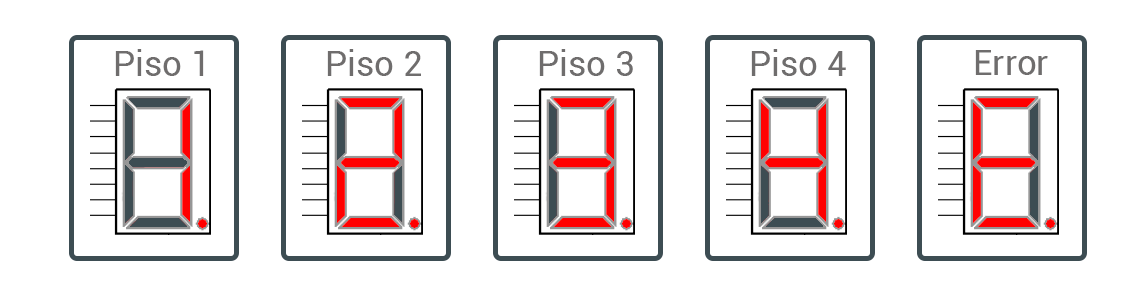
\includegraphics[width = 1\textwidth ]{displays7s}
		    \caption{Salida en los displays de 7 segmentos}
		    \label{fig:displays7s}
	\end{figure}
    
    La interfaz, entradas y salidas, de este bloque se puede ver su representación en la Figura \ref{fig:BloqueDecodificador7seg}:
    
    \begin{figure}[H]
		    \centering
		    \includegraphics[width = 0.7\textwidth ]{BloqueDecodificador}
		    \caption{Diagrama Interfaz Bloque Decodificador a 7 segmentos}
		    \label{fig:BloqueDecodificador7seg}
	\end{figure}
\subsection{Bloque \textit{Divisor de frecuencia}:}

\subsection{Bloque \textit{PistoActual}:}
    Como se ha dicho anteriormente en cada piso hay un final de carrera que detecta el paso del ascensor. El prpósito de este bloque es el de filtrar dicha entrada de 4 bits. En este caso lo que interesa es saber en que piso estoy o en que piso he estado por última vez. Cuando el ascensor se encuentra entre dos pisos la entrada de los sensores será \textit{0000}, este bloque lo que hará será mantener en la salida del mismo el último piso por el que haya pasado el ascensor. \\ 
    
    Como se puede apreciar en el siguiente diagrama este bloque tiene una entrada, un vector de 4 bits (los finales de carrera de cada piso) y una salida, también de 4 bits, codificando el piso en el que se encuentra actualmente. \\ 
    
    Se puede consultar dicha codificación en el Cuadro (\ref{tab:tabla1ApendiceA}) del Apéndice \ref{app:codEntSal}. \\ 
    
    La interfaz, entradas y salidas, de este bloque se puede ver su representación en la Figura \ref{fig:BloquePisoActual}:
    
    \begin{figure}[H]
		    \centering
		    \hspace*{-1.8cm}
		    \includegraphics[width = 0.6\textwidth ]{BloquePisoActual}
		    \caption{Diagrama Bloque PisoActual}
		    \label{fig:BloquePisoActual}
	\end{figure}
	
	Se puede consultar el código VHDL de este módulo en el Apartado \ref{code:PisoActual} así como el código de su testbench correspondiente en el Apartado \ref{code:PisoActual_tb}.

\subsection{Bloque \textit{Bloqueador pisoVoy}:}
    
    La interfaz, entradas y salidas, de este bloque se puede ver su representación en la Figura \ref{fig:BloqueBloqueadorPisoVoy}:
    
    
    \begin{figure}[H]
		    \centering
		    \hspace*{-1.8cm}
		    \includegraphics[width = 0.6\textwidth ]{BloqueBloqueadorPisoVoy}
		    \caption{Diagrama Bloque Bloqueador PisoVoy}
		    \label{fig:BloqueBloqueadorPisoVoy}
	\end{figure}
	
\subsection{Código Bloque \textit{Decodificador Binario a Decimal}:} 
	En este bloque se traduce la señal binaria que codifica tanto el piso actual como el piso de destino a decimal para su posterior comparación.
	Se puede consultar dicha codificación en el Cuadro (\ref{tab:tabla1ApendiceA}) del Apéndice \ref{app:codEntSal}. \\ 
	
\subsection{Bloque \textit{Comparador}:}

    La interfaz, entradas y salidas, de este bloque se puede ver su representación en la Figura \ref{fig:BloqueComparador}:
    
    \begin{figure}[H]
		    \centering
		    \includegraphics[width = 0.6\textwidth ]{BloqueComparador}
		    \caption{Diagrama Bloque Comparador}
		    \label{fig:BloqueComparador}
	\end{figure}